\documentclass[portrait,a0]{a0poster}

% definovanie kompilatora (magic comment):


% ============== PREAMBULA ==============
% (nacitanie balikov a podobne)
% ============== PREAMBULA ==============
% (nacitanie balikov a podobne)
% Ctrl+klik na balik zobrazi dokumentaciu k baliku (v TeXstudiu)
% Je tu vela uzitocnych balikov ak ale nejaky nepotrebujete, zakomentujte ho

%definovanie verzie dokumentu (pdf/tlacena)
\usepackage{etoolbox}
\newbool{printVersion} % premenna pre volbu verzie
%\booltrue{printVersion} % tlacena: odkomentovat, pdf: nechat zakomentovanie


% geometria a formatovanie stran
\pagestyle{plain} % defaultny styl stran (plain/headings/empty/myheadings)
\ifbool{printVersion}{
	\usepackage[top=2.5cm, bottom=2.5cm, left=3.5cm, right=2cm]{geometry} % odporucane okraje
}{
	\usepackage[top=2.5cm, bottom=2.5cm, left=2.75cm, right=2.75cm]{geometry} % okraje vhodnejsie do pdf (rovnaka sirka vlavo/vpravo) 
}

% jazyk
\usepackage[main=slovak,english]{babel}  % primarny jazyk: SK, dalsie jazyky: EN


% bibliografia
\usepackage[style=iso-numeric,backend=bibtex,giveninits=true,sorting=nyt]{biblatex}
\addbibresource{literatura.bib}


% fromatovanie
\usepackage{indentfirst} % odsadenie prveho odstavca
\usepackage{enumitem} % číslovanie ((a),(b),(c),... i), ii), iii),...)
\usepackage[small]{caption} % male popisy obrazkov


% grafika
\usepackage{graphicx} % obrazky
\usepackage{subcaption} % podobrazky (subfigure)
\graphicspath{ {./figures/} } % priecinok s obrazkami
\usepackage{wrapfig} % obrazky obtekane textom
\usepackage[dvipsnames]{xcolor} % farby (dvipsnames pridava dalsie farby)
\usepackage{colortbl} % farebne tabulky
\usepackage{multirow} % treba pre merge-ovanie budniek v tabulkach

\usepackage{pdfpages} % vlozenie stran z ineho pdf (musi byt za graphics)


% matematika
\usepackage{mathtools} % rozsirenie zakladneho matematickeho balika amsmath
\usepackage{amssymb} % dalsie symboly a fonty (napriklad pre mnozinu realnych cisel)
\usepackage[locale=DE]{siunitx} % jednotky SI

% Definície, Vety, Dôkazy...
\usepackage{amsthm}
\theoremstyle{definition}
\newtheorem{thm}{Veta}[chapter]
\newtheorem{defn}[thm]{Definícia}
\newtheorem{lem}[thm]{Lemma}
\newtheorem{cor}[thm]{Dôsledok}
\newtheorem{rem}[thm]{Poznámka}
\newtheorem{exmp}[thm]{Príklad}


% pseudokod a kod
\usepackage[czech]{algorithm2e} % pseudokody/algoritmy
\usepackage{listings} % vkladanie kodu


% hyperreferencia
\ifbool{printVersion}{
	% hyperreferencia v tlacenej verzii
	\usepackage[hidelinks]{hyperref} % hyperreferencia
}{
	% hyperreferencia v pdf verzii
	\usepackage{hyperref} % hyperreferencia
	\hypersetup{colorlinks, % farby linkov
		citecolor = red,
		linkcolor = blue,
		urlcolor = blue}
}


% Ked uz je praca dlha, pre urychlenie kompilacie sa oplati vkladat len niektore kapitoly
%\includeonly{
	%%	Uvod,
	%%	Kapitola1,
	%%	Kapitola2,
	%	Kapitola3,
	%%	Zaver
	%}


% ============== DOKUMENT ==============
\begin{document}
	\renewcommand{\baselinestretch}{1.5} % riadkovanie- mozete upravit
	\fontsize{25pt}{20pt} % velkost fontu a medzier - mozete opravit
	\selectfont
	
	% ====== HLAVICKA ======
	\centerline{\includegraphics[width=\paperwidth]{header/header.pdf}}
	\centerline{\huge \textsc{\textbf{Názov práce}}}
	\centerline{\huge \textsc{\textbf{(prípadne druhý riadok názvu)}}}
	\vskip 1cm 
	\centerline{\Large Meno Priezvisko}
	\vskip 0.5cm
	\leaders\vrule width \linewidth\vskip 3pt

	% ====== JADRO ======
	\begin{multicols}{3} % cislom sa nastavuje pocet stplcov

	\section*{Na čo je dobrý poster}
	
	Pri odovzdávaní práce do AIS sa odovzdáva aj poster. Môžete ho chápať ako vizuálnu \uv{upútavku} na vašu prácu. Postery bývajú niekedy vystavené na chodbách fakulty a prezentujú práce našich študentov. Niekoľko posterov študentov je aj na chodbách našej katedry. Využívame ich aj pri prezentácii MPM pre potenciálnych záujemcov o štúdium, napríklad na dni otvorených dverí SvF.
	
	Niekoľko príkladov posterov nájdete v priečinku \verb*|poster\inspiracia|. Nechápte to v zmysle \uv{takto to má byť}, naozaj to berte len ako inšpiráciu, čo robili študenti MPM v minulosti.
	
	Je dobré sa zamerať na estetické, jasné a čitateľné podanie vašej práce. Veľmi dôležité sú obrázky a kľúčové vzorce, text by mal byť v rámci možností stručný, ale jasný. Predstavte si, že prechádzate po chodbe plnej posterov. Ktorý poster vás zaujme? Väčšinu ľudí zrejme ten, čo má pekné a zaujímavé obrázky. Až keď sa priblížite, všimnete si vzorce a prípadne sa zahĺbite do čítania textu.
	
	Táto šablóna je graficky jednoduchá, vyniknúť by mal obsah, ktorý doplníte. Dá sa s tým vyhrať, môžete skúsiť zmeniť farbu pozadia, doplniť nejaké rámiky. Množstvo inšpirácie nájdete na stránke \href{https://www.latextemplates.com/cat/conference-posters}{\textcolor{blue}{latextemplates.com}}, či na  \href{https://www.overleaf.com/gallery/tagged/poster}{\textcolor{blue}{stránke Overleaf-u}}, kde je aj veľa \href{https://www.overleaf.com/learn/latex/Posters}{\textcolor{blue}{tipov na tvorbu posteru}}. Vyhnite sa ale príliš výraznému pozadiu a grafike, ktorá \uv{zabije} obsah. Poster sa dá urobiť aj v PowerPointe, avšak pre väčšinu študentov bude zrejme jednoduchšie sem iba z LaTeX-u nakopírovať časti práce a vhodne ich upraviť/zjednodušiť.
	
	Niekoľko poznámok:
	\begin{itemize}
		\item Súbor \verb|header\header.tex| nijak neupravujte.
		\item Upravte názov práce a meno.
		\item Otvorte súbor \verb|footer\footer.tex|, upravte ho a skompilujte. Fotku \verb|footer\foto.JPG| vymeňte za svoju fotku (napr. z AIS). Fotka ale nie je na našej katedre vyžadovaná, nemusíte ju tam dávať. V tom prípade stačí príslušný riadok zakomentovať.
		\item Upravte jadro postera, je to naozaj úplne na vás, môžete meniť formátovnie, počet odstavcov (odporúčané sú 3), riadkovanie, či veľkosť písma (ale pozor na príliš malé/veľké písmo, interval 20pt -- 30pt je v poriadku).
		\item Snažte sa využiť celú plochu postera.
	\end{itemize}
	
	\section*{Obrázky}
	Obrázky sú veľmi dôležité, keďže sú v posteri hlavným prvkom, ktorý vizuálne prezentuje vašu prácu. Väčšinou sa používa podmnožina obrázkov z práce. Treba ich starostlivo zvoliť tak, aby boli dostatočne ilustratívne. Podobne ako pri práci, aj pri posteri je dobré mať obrázky, ktoré chcete vložiť do posteru, pokope v priečinku. V preambule je cesta k priečinku nastavená pomocou príkazu 
	\verb|\graphicspath{ {./figures/} }|.

	\begin{center}
		\includegraphics[width=\linewidth]{klavir2}
		\captionof{figure}{Označenia tónov na klaviatúre.}
		\label{fig:klavir}
	\end{center}
	
	\subsection*{Vkladanie obrázkov}
	
	Hlavná zmena oproti práci je, že v posteri sa nedajú používať plávajúce (float) prostredia (\verb|figure|, \verb|table|). Takže obrázky a tabuľky treba vkladať inak. Nižšie je niekoľko príkladov. Jednoduchý obrázok na šírku textu v stĺpci je na Obr.~\ref{fig:klavir}. Všimnite si, že popis sa robí cez \verb|\captionof{figure}{...}|. Popisy obrázkov sa ale kvôli šetreniu priestoru môžu aj vynechať.
	
	\begin{center}
		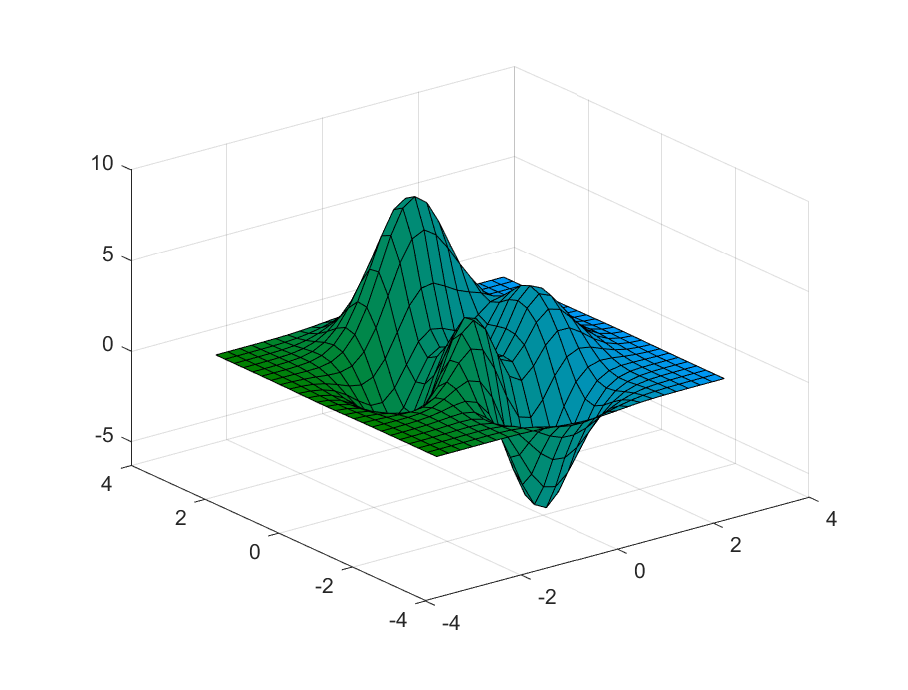
\includegraphics[width=0.7\linewidth]{matlab_3D}
		
		\textit{Popisy obrázkov môžu byť aj nečíslované.}
	\end{center}

	\begin{center}
		\includegraphics[height=6cm]{fig_hyperbolicky_paraboloid}
		\quad
		\includegraphics[height=6cm]{st_chas_framing}
		\captionof{figure}{Graf funkcie $f(x,y)=xy$ a konštruovanie strechy v tvare hyperbolického paraboloidu.} \label{fig:hyperbolicky_paraboloid}
	\end{center}
	
	Príklad dvoch obrázkov vložených vedľa seba (s jedným popisom) vidíme na Obrázku~\ref{fig:hyperbolicky_paraboloid}. Analogicky sa dajú urobiť aj 3 obrázky vedľa seba, prípadne mriežka obrázkov (napr. 4x2, ako vidíme na Obrázku~\ref{fig:bumpy_sphere}). Ak ale chceme, aby každý obrázok mal svoje číslo a popis, môžeme to urobiť napríklad tak, ako vidíme na príklade Obrázkov~\ref{fig:vzduchovod_geom}~a~\ref{fig:vzduchovod_mesh}.
	
	\begin{center}
		%	\vspace{-5pt}
		\centering
		\includegraphics[width=0.35\linewidth]{bumpy_noRed_level5_tstep0_FT.png}
		\hspace{0.1\linewidth}
		\includegraphics[width=0.35\linewidth]{bumpy_noRed_level5_tstep0_FT.png}
		\newline
		\includegraphics[width=0.35\linewidth]{bumpy_noRed_level5_tstep20.png}
		\hspace{0.1\linewidth}
		\includegraphics[width=0.35\linewidth]{bumpy_omega100_level5_tstep20.png}
		\newline
		\includegraphics[width=0.35\linewidth]{bumpy_noRed_level5_tstep50.png}
		\hspace{0.1\linewidth}
		\includegraphics[width=0.35\linewidth]{bumpy_omega100_level5_tstep50.png}
		\newline
		\includegraphics[width=0.35\linewidth]{bumpy_noRed_level5_tstep128.png}
		\hspace{0.1\linewidth}
		\includegraphics[width=0.35\linewidth]{bumpy_omega100_level5_tstep128.png}
		\newline
		\vspace{-20pt}
		\captionof{figure}{Príklady obrázkov z ParaView.}\label{fig:bumpy_sphere} 
		%\vspace{-10pt}
	\end{center}

	\begin{center}
		\vspace{-5pt}
		\begin{minipage}{.5\linewidth}
			\centering
			\includegraphics[width=0.95\linewidth]{vzduchovod1}
			\vspace{-5pt}
			\captionof{figure}{Obrázok z ANSYS-u.}
			\label{fig:vzduchovod_geom}
		\end{minipage}%
		\begin{minipage}{.5\linewidth}
			\centering
			\includegraphics[width=0.95\linewidth]{vzduchovod2}
			\vspace{-5pt}
			\captionof{figure}{Obrázok z ANSYS-u.}
			\label{fig:vzduchovod_mesh}
		\end{minipage}
		\vspace{-5pt}
	\end{center}
	
	Dajú sa použiť aj obrázky obtekané textom (wrapfigure), ale z nejakých dôvodov je obtiažnejšie nastaviť rozmery obrázka tak, ako človek chce.

	\begin{wrapfigure}{l}{0.3\linewidth}
		\centering
		\includegraphics[width=1.5\linewidth]{parabola}
		\caption{Wrapfigure.}
		\label{fig:parabola}
	\end{wrapfigure}
	\textit{Lorem ipsum dolor sit amet, consectetur adipiscing elit. Cras mollis metus metus. Nam eget sapien elementum, pharetra arcu ut, congue tortor. Nulla non tortor ullamcorper, pretium turpis ac, accumsan erat. Vestibulum porttitor leo in arcu laoreet, vitae ullamcorper massa blandit. Vestibulum fermentum euismod dui, vel blandit dolor. Maecenas aliquam pharetra nunc, quis mollis turpis sodales non.}
	

	\section*{Vzorce}
	
	V posteri je dobré uviesť kľúčové vzorce, ktoré používate v práci. Netreba zachádzať do úplných detailov (napríklad uvádzať celú numerickú schému), aby ste poster príliš nezahltili. Nižšie je niekoľko vzorcov (nie je nutné, aby boli číslované). Vzorec \eqref{eq:Gauss} je Gaussova veta
	\begin{equation}\label{eq:Gauss}
		\int\limits_{V} \nabla\cdot\vec{F}\,dx = \int\limits_{\partial V} \vec{F}\cdot\vec{n}\,dS.
	\end{equation}
	Tu sú Maxwellove rovnice
	\begin{subequations}
		\label{eq:Maxwell}
		\begin{align}
			\nabla\cdot\mathbf{D}  & =\rho,    \label{eq:Maxwell_1}                                               \\
			\nabla\times\mathbf{E} & = -\frac{\partial \mathbf{B}}{\partial t},  \label{eq:Maxwell_2}             \\
			\nabla\cdot\mathbf{B}  & =0,    \label{eq:Maxwell_3}                                                  \\
			\nabla\times\mathbf{H} & = \frac{\partial \mathbf{D}}{\partial t} + \mathbf{J}.  \label{eq:Maxwell_4}
		\end{align}
	\end{subequations}
	
	
	\section*{Tabuľky}
	
	Keďže prostredie \verb|table| je plávajúce, nemôžeme ho použiť a do posteru treba vložiť tabuľku inak. Príkladom správne vloženej tabuľky je Tab.~\ref{tab:resultsDDFV}.
	
	\begin{center}
		\captionof{table}{The $L^2$ EOC for the case with no redistribution.}
		\begin{tabular}{rlrrr}
			\hline
			$n_V$ & $\tau$     & $N$ & $ L^2\mbox{ error}$ &  EOC \\ \hline
			122 & 0.04       &   2 &            1.43e-02 &      \\
			482 & 0.01       &   8 &            3.35e-03 & 2.10 \\
			1922 & 0.0025     &  32 &            8.07e-04 & 2.05 \\
			7682 & 0.000625   & 128 &            1.95e-04 & 2.05 \\
			30722 & 0.00015625 & 512 &            4.64e-05 & 2.07 \\ \hline
		\end{tabular}
		\label{tab:resultsDDFV}
	\end{center}
	
	
	\section*{Videá}
	
	Ak máte k práci nejaké užitočné dodatočné materiály, napríklad videá, či zvukové nahrávky, je vhodné ich zavesiť niekam online (napríklad vytvoriť \href{https://www.youtube.com/playlist?list=PLI7npCkiqdtxGtS1VIZW3aDIIJM1EJoFR}{playlist na YouTube}) a pridať QR kód niekam na spodok postera.
	\begin{center}
		\includegraphics[height=4.8cm]{figures/QRcode}
		\label{fig:qr}
	\end{center}
	
	
	\section*{Citovanie literatúry}
	
	Citovať literatúru na posteri nebýva zvykom, ani to nie je potrebné (obmedzený priestor postera sa dá využiť lepšie), ale ak z nejakého dôvodu potrebujete uviesť nejakú kľúčovú literatúru ~\cite{eymard}, \cite{Handlovicova}, urobíte to rovnako ako v práci.
	
	% ====== Bibliografia a prilohy ======
	%	\nocite{*} % Vypise v bibliografii aj zroje, ktore neboli citovane
	\printbibliography

	%	\vspace*{50mm} % ak vam nedarilo vvyuzit celu plochu postera, da sa pomoct tymto bielym miestom 
	\end{multicols}
	\vfill

	% ====== PATA POSTERA ======
	\centerline{\includegraphics[width=\paperwidth]{footer/footer.pdf}}
\end{document}